% unit: u07
% sources: sources/090-column-space-and-nullspace.txt, sources/142-column-space-and-nullspace.txt, sources/143-mit18-06scf11-ses1-6sum-pdf-download-file.txt, sources/144-vector-subspaces.txt, sources/145-mit18-06scf11-ses1-6prob-pdf-download-file.txt, sources/146-mit18-06scf11-ses1-6sol-pdf-download-file.txt, short_plan.json (s02)
\section{Column space and nullspace}\label{sec:u07}

Every matrix carries two subspaces that answer the two basic questions about
$A\vb{x}=\vb{b}$. The \emph{column space} $\Col{A}$ answers ``for which $\vb{b}$ is there a
solution?'': exactly those $\vb{b}$ that are combinations of the columns. The
\emph{nullspace} $\Nul{A}$ answers ``how many solutions are there?'': any two solutions differ
by a vector that $A$ sends to zero. The two subspaces are built in opposite ways. The column
space is \emph{spanned}: we are handed some vectors and take all their combinations. The
nullspace is \emph{cut out by equations}: we are told the conditions $A\vb{x}=\vb{0}$ and must
find which vectors satisfy them. This section works both out for small examples by inspection;
Section~\ref{sec:u08} gives the systematic method by elimination.

\subsection{Unions and intersections of subspaces}

Recall that a subspace is a nonempty set of vectors closed under addition and scalar
multiplication (Definition~\ref{def:u06-subspace}); equivalently, for any $\vb{v},\vb{w}$ in
the subspace and any numbers $c,d$, the combination $c\vb{v}+d\vb{w}$ is in it. In $\R^3$ a plane
$P$ through the origin and a line $L$ through the origin are subspaces. What about combining
them?

\emph{The union is usually not a subspace.} Take $P$ to be the $x_1x_2$-plane (vectors
$(x_1,x_2,0)$) and $L$ the $x_3$-axis. Then $(1,0,0)\in P$ and $(0,0,1)\in L$, but their sum
$(1,0,1)$ is in neither, so $P\cup L$ is not closed under addition.

\begin{theorem}[Intersections of subspaces are subspaces]\label{thm:u07-intersection}
If $S$ and $T$ are subspaces of a vector space $V$, then $S\cap T$, the set of vectors lying
in both, is a subspace of $V$.
\end{theorem}

\begin{proof}
$\vb{0}$ lies in both $S$ and $T$ (Proposition~\ref{prop:u06-zero}), so $S\cap T$ is nonempty.
Let $\vb{v},\vb{w}\in S\cap T$ and $c,d\in\R$. Since $\vb{v},\vb{w}\in S$ and $S$ is a subspace,
$c\vb{v}+d\vb{w}\in S$. Since $\vb{v},\vb{w}\in T$ and $T$ is a subspace, $c\vb{v}+d\vb{w}\in T$.
So $c\vb{v}+d\vb{w}\in S\cap T$.
\end{proof}

For the plane and line above, $P\cap L=\{\vb{0}\}$, the zero subspace. Intersecting adds
requirements, so the intersection is usually smaller, but it is always a subspace.
(Exercise~\ref{ex:u07-sum} shows that the right way to combine two subspaces into a bigger
one is their sum $S+T$, not their union.)

\subsection{The column space decides solvability}

Our example is the $4\times3$ matrix
\begin{equation}\label{eq:u07-A}
  A=\begin{bmatrix} 1&1&2\\ 2&1&3\\ 3&1&4\\ 4&1&5\end{bmatrix},\qquad
  A\vb{x}=x_1\begin{bmatrix}1\\2\\3\\4\end{bmatrix}+x_2\begin{bmatrix}1\\1\\1\\1\end{bmatrix}
         +x_3\begin{bmatrix}2\\3\\4\\5\end{bmatrix}=\begin{bmatrix}b_1\\b_2\\b_3\\b_4\end{bmatrix}.
\end{equation}
Its columns are vectors in $\R^4$, so its column space
$\Col{A}=\{A\vb{x}:\vb{x}\in\R^3\}$ (Definition~\ref{def:u06-colspace}) is a subspace of
$\R^4$. These are four equations in only three unknowns, and we should not expect a solution
for every $\vb{b}$: the combinations of three vectors cannot fill four-dimensional space.
But some right-hand sides are fine, and they are exactly the vectors in the column space.

\begin{theorem}[Solvability]\label{thm:u07-solvable}
$A\vb{x}=\vb{b}$ has a solution if and only if $\vb{b}$ is in the column space $\Col{A}$.
\end{theorem}

\begin{proof}
$A\vb{x}$ is the combination of the columns with weights $x_1,\dots,x_n$. If a solution
$\vb{x}$ exists, $\vb{b}=A\vb{x}$ is such a combination, so $\vb{b}\in\Col{A}$. Conversely,
if $\vb{b}$ is a combination $x_1\vb{a}_1+\cdots+x_n\vb{a}_n$, those weights form a solution
$\vb{x}$.
\end{proof}

A good way to find vectors in $\Col{A}$ is to choose $\vb{x}$ first and compute $\vb{b}$. The
right side $\vb{b}=\vb{0}$ is always reached (by $\vb{x}=\vb{0}$); $\vb{b}=(1,2,3,4)$ is
column~1, reached by $\vb{x}=(1,0,0)$; $\vb{b}=(1,1,1,1)$ is column~2, reached by
$\vb{x}=(0,1,0)$.

How big is $\Col{A}$? Column~3 is the sum of columns~1 and~2, so it contributes nothing new:
by Proposition~\ref{prop:u01-dependent} every combination of all three columns is already a
combination of the first two. Columns~1 and~2 are not on one line, so their combinations form
a plane. Hence \emph{$\Col{A}$ is a two-dimensional subspace (a plane) of $\R^4$}. We could
equally have thrown away column~1, since column~1 $=$ column~3 $-$ column~2; the convention
(made precise in Section~\ref{sec:u08}) is to keep the earliest columns that are not
combinations of earlier ones, the \emph{pivot columns}.

\begin{example}[Equations for the column space]\label{ex:u07-colspace}
Which $\vb{b}\in\R^4$ lie in $\Col{A}$? We need $\vb{b}=x_1(1,2,3,4)+x_2(1,1,1,1)$, that is,
$b_i=i\,x_1+x_2$ for $i=1,2,3,4$: the components of $\vb{b}$ must form an arithmetic
progression. That is two equations:
\[
  \Col{A}=\{\vb{b}\in\R^4:\ b_1-2b_2+b_3=0\ \text{and}\ b_2-2b_3+b_4=0\}.
\]
Indeed each column passes both tests (for column~3: $2-6+4=0$ and $3-8+5=0$), and the tests are
preserved by combinations. Conversely, if $\vb{b}$ passes both tests then the differences
$b_2-b_1=b_3-b_2=b_4-b_3$ share a common value $d$, and
$\vb{b}=d\,(1,2,3,4)+(b_1-d)\,(1,1,1,1)$. So $A\vb{x}=(2,3,4,5)$ is solvable (it is column~3),
while $A\vb{x}=(1,2,3,5)$ is not, because $b_2-2b_3+b_4=2-6+5=1\neq0$.
\end{example}

\subsection{The nullspace}

\begin{definition}[Nullspace]\label{def:u07-nullspace}
The \emph{nullspace} of an $m\times n$ matrix $A$ is the set of all solutions of
$A\vb{x}=\vb{0}$:
\[
  \Nul{A}=\{\vb{x}\in\R^n:\ A\vb{x}=\vb{0}\}.
\]
\end{definition}

The column space contains right-hand sides $\vb{b}\in\R^m$; the nullspace contains inputs
$\vb{x}\in\R^n$. For the $4\times3$ example, $\Col{A}\subseteq\R^4$ while
$\Nul{A}\subseteq\R^3$.

\begin{theorem}[The nullspace is a subspace]\label{thm:u07-nullspace}
For every $m\times n$ matrix $A$, $\Nul{A}$ is a subspace of $\R^n$.
\end{theorem}

\begin{proof}
$A\vb{0}=\vb{0}$, so $\vb{0}\in\Nul{A}$. If $A\vb{v}=\vb{0}$ and $A\vb{w}=\vb{0}$, then by the
distributive law $A(\vb{v}+\vb{w})=A\vb{v}+A\vb{w}=\vb{0}+\vb{0}=\vb{0}$, and for any scalar
$c$, $A(c\vb{v})=c\,A\vb{v}=c\,\vb{0}=\vb{0}$. So $\Nul{A}$ is closed under addition and scalar
multiplication.
\end{proof}

\begin{example}[A nullspace that is a line]\label{ex:u07-nullspace}
For $A$ in \eqref{eq:u07-A}, the relation column~1 $+$ column~2 $-$ column~3 $=\vb{0}$ says
that $(1,1,-1)\in\Nul{A}$, and so is every multiple $c(1,1,-1)$. Are there other solutions?
Write $\vb{a}_1,\vb{a}_2$ for the first two columns. Since $\vb{a}_3=\vb{a}_1+\vb{a}_2$,
\[
  A\vb{x}=x_1\vb{a}_1+x_2\vb{a}_2+x_3(\vb{a}_1+\vb{a}_2)=(x_1+x_3)\,\vb{a}_1+(x_2+x_3)\,\vb{a}_2 .
\]
Because $\vb{a}_1$ and $\vb{a}_2$ are not parallel, this combination is zero only when both
weights are zero: $x_1=-x_3$ and $x_2=-x_3$. So $\vb{x}=-x_3(1,1,-1)$, and
\[
  \Nul{A}=\{c\,(1,1,-1):c\in\R\},
\]
a line through the origin in $\R^3$.
\end{example}

\subsection{The solutions of \texorpdfstring{\(A\vb{x}=\vb{b}\)}{Ax = b} are a shifted nullspace}

Now take a right-hand side that is not zero, say $\vb{b}=(1,2,3,4)$. One solution is
$\vb{x}=(1,0,0)$; another is $(0,-1,1)$, since $-$column~2 $+$ column~3 $=(1,2,3,4)$. The
solutions do \emph{not} form a subspace: $\vb{x}=\vb{0}$ is not a solution, because
$A\vb{0}=\vb{0}\neq\vb{b}$. Their structure is described next.

\begin{proposition}[All solutions]\label{prop:u07-allsolutions}
Suppose $A\vb{x}_p=\vb{b}$. Then the solutions of $A\vb{x}=\vb{b}$ are exactly the vectors
$\vb{x}=\vb{x}_p+\vb{x}_n$ with $\vb{x}_n\in\Nul{A}$.
\end{proposition}

\begin{proof}
If $\vb{x}_n\in\Nul{A}$, then $A(\vb{x}_p+\vb{x}_n)=\vb{b}+\vb{0}=\vb{b}$. Conversely, if
$A\vb{x}=\vb{b}$, then $A(\vb{x}-\vb{x}_p)=\vb{b}-\vb{b}=\vb{0}$, so $\vb{x}_n=\vb{x}-\vb{x}_p$
is in $\Nul{A}$ and $\vb{x}=\vb{x}_p+\vb{x}_n$.
\end{proof}

For our example the solutions of $A\vb{x}=(1,2,3,4)$ are $(1,0,0)+c(1,1,-1)$: a line parallel
to the nullspace but shifted away from the origin (Figure~\ref{fig:u07-shifted}); $c=-1$ gives
$(0,-1,1)$. Section~\ref{sec:u09} builds on this to find the complete solution of any system.

\begin{figure}[ht]
\centering
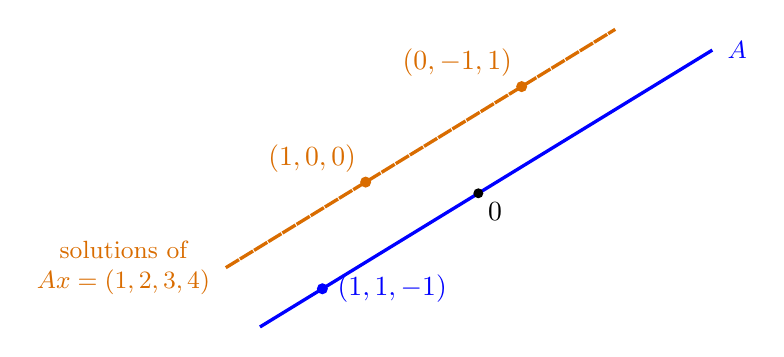
\begin{tikzpicture}
\begin{axis}[view={200}{25}, width=9cm, height=7cm, axis lines=none,
  xmin=-1.6, xmax=2.2, ymin=-1.8, ymax=1.8, zmin=-1.8, zmax=1.8, clip=false]
  \addplot3[very thick, blue, domain=-1.5:1.4, samples=2] ({x},{x},{-x});
  \addplot3[very thick, dashed, orange!85!black, domain=-1.6:0.9, samples=2] ({1+x},{x},{-x});
  \fill (0,0,0) circle (1.8pt) node[below right] {$\vb{0}$};
  \fill[blue] (1,1,-1) circle (2pt) node[right=2pt] {$(1,1,-1)$};
  \fill[orange!85!black] (1,0,0) circle (2pt) node[above left] {$(1,0,0)$};
  \fill[orange!85!black] (0,-1,1) circle (2pt) node[above left] {$(0,-1,1)$};
  \node[blue,font=\small] at (-1.5,-1.5,1.5) [right=2pt] {$\Nul{A}$};
  \node[orange!85!black,font=\small,align=center] at (1.9,0.9,-0.9) [left=2pt] {solutions of\\ $A\vb{x}=(1,2,3,4)$};
\end{axis}
\end{tikzpicture}
\caption{For the $4\times3$ matrix $A$ of \eqref{eq:u07-A}, the nullspace is the line through
$(1,1,-1)$ (solid). The solutions of $A\vb{x}=(1,2,3,4)$ form the parallel line through
$(1,0,0)$ and $(0,-1,1)$ (dashed): one particular solution plus the whole nullspace. It does
not pass through the origin, so it is not a subspace.}\label{fig:u07-shifted}
\end{figure}

The two examples show the two ways of describing a subspace. For $\Col{A}$ we were
\emph{given} vectors (the columns) and took all their combinations. For $\Nul{A}$ we were given
\emph{equations} ($A\vb{x}=\vb{0}$) and had to discover which vectors satisfy them; the answer
turned out to be all combinations of one vector. Example~\ref{ex:u07-colspace} went the other
way, describing $\Col{A}$ by equations. Turning one description into the other is a recurring
task of the course.

\begin{trap}
Keep the spaces apart: for an $m\times n$ matrix, $\Col{A}$ lies in $\R^m$ (vectors as long as
a column) while $\Nul{A}$ lies in $\R^n$ (vectors with one entry per column). And the solution
set of $A\vb{x}=\vb{b}$ with $\vb{b}\neq\vb{0}$ is never a subspace, even when it looks like a
line or plane: it is a copy of $\Nul{A}$ shifted off the origin.
\end{trap}

\subsection{What a matrix keeps and what it crushes}

The next example previews the main theorem of Part~I. A matrix sends some input directions to
zero; those directions form the nullspace, and the information they carry is lost.

\begin{example}[What the matrix crushes]\label{ex:u07-crush}
Let $A=\begin{bmatrix} 1&2&2\\ 2&4&4\end{bmatrix}$: two outputs, three inputs ($m=2$,
$n=3$).
\begin{enumerate}
  \item \emph{Eliminate.} Row~2 $-$ 2 row~1 $=(0,0,0)$, leaving one pivot. So $A\vb{x}=\vb{0}$ is
    the single equation $x_1+2x_2+2x_3=0$. (The number of pivots, here $r=1$, is the
    \emph{rank}; see Section~\ref{sec:u08}.)
  \item \emph{The nullspace is a plane.} Choosing $x_2,x_3$ freely and setting
    $x_1=-2x_2-2x_3$ gives every solution:
    $\vb{x}=x_2(-2,1,0)+x_3(-2,0,1)$. The two \emph{special solutions}
    $\vb{s}_1=(-2,1,0)$ and $\vb{s}_2=(-2,0,1)$ satisfy $A\vb{s}_1=A\vb{s}_2=(0,0)$, so $\Nul{A}$
    is the plane of their combinations, of dimension $2=n-r$.
  \item \emph{The row is perpendicular to that plane.} The row $(1,2,2)$ has dot product
    $-2+2+0=0$ with $\vb{s}_1$ and $-2+0+2=0$ with $\vb{s}_2$. The \emph{row space}, all
    multiples of $(1,2,2)$, is a line (dimension $r=1$) perpendicular to $\Nul{A}$.
  \item \emph{The nullspace part is crushed.} Take $\vb{x}=(-1,3,2)=(1,2,2)+\vb{s}_1$. Then
    $A\vb{x}=(-1+6+4,\,-2+12+8)=(9,18)$, exactly $A(1,2,2)=(1+4+4,\,2+8+8)=(9,18)$: adding
    $\vb{s}_1$ changed nothing.
  \item \emph{Outputs.} Every column is a multiple of $(1,2)$, so $\Col{A}$ is the line through
    $(1,2)$ in $\R^2$ (dimension $r=1$). The perpendicular line through $(2,-1)$ is the
    \emph{left nullspace} (dimension $m-r=1$): it contains the vectors $\vb{y}$ with
    $A\T\vb{y}=\vb{0}$, since $(2,-1)\cdot(1,2)=0$.
\end{enumerate}
The input space splits as $\R^3=$ row-space line $+$ nullspace plane, $1+2=3$; the output
space splits as $\R^2=$ column-space line $+$ left-nullspace line, $1+1=2$.
Figure~\ref{fig:u07-crush} draws both. Sections~\ref{sec:u10} and~\ref{sec:u11} prove that
these dimension counts, $r+(n-r)=n$ and $r+(m-r)=m$, hold for every matrix.
\end{example}

\begin{figure}[ht]
\centering
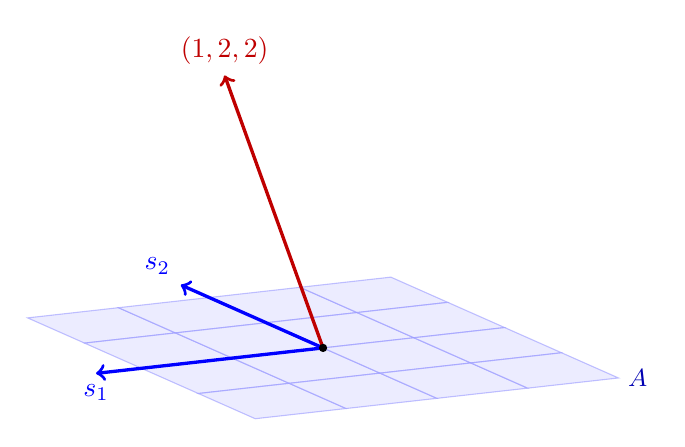
\begin{tikzpicture}
\begin{axis}[view={-50}{15}, width=9.5cm, height=9.5cm, axis lines=none,
  xmin=-2, xmax=2, ymin=-2, ymax=2, zmin=-2, zmax=2, clip=false,
  unit vector ratio=1 1 1]
  \addplot3[surf, shader=faceted, colormap={single}{color=(blue!12) color=(blue!12)},
    faceted color=blue!40, opacity=0.6, samples=5, domain=-0.8:0.8, y domain=-0.8:0.8]
    ({-2*x-2*y},{x},{y});
  \draw[->,very thick,blue] (0,0,0) -- (-2,1,0) node[below] {$\vb{s}_1$};
  \draw[->,very thick,blue] (0,0,0) -- (-2,0,1) node[above left] {$\vb{s}_2$};
  \draw[->,very thick,red!75!black] (0,0,0) -- (1,2,2) node[above] {$(1,2,2)$};
  \fill (0,0,0) circle (1.5pt);
  \node[blue!70!black,font=\small] at (3.2,-0.8,-0.8) [right] {$\Nul{A}$};
\end{axis}
\end{tikzpicture}
\qquad
\begin{tikzpicture}[scale=0.9,>=Stealth]
  \draw[->] (-2.6,0) -- (2.8,0) node[right] {$y_1$};
  \draw[->] (0,-2.4) -- (0,3.2) node[above] {$y_2$};
  \draw[very thick,blue] (-1.2,-2.4) -- (1.55,3.1) node[right] {$\Col{A}$};
  \draw[very thick,red!75!black] (-2.6,1.3) -- (2.8,-1.4) node[below] {left nullspace};
  \draw[->,very thick,blue] (0,0) -- (1,2) node[right] {$(1,2)$};
  \draw[->,very thick,red!75!black] (0,0) -- (2,-1) node[above right] {$(2,-1)$};
  \fill (0,0) circle (1.5pt);
\end{tikzpicture}
\caption{The matrix $A=\begin{bmatrix} 1&2&2\\ 2&4&4\end{bmatrix}$. Left (inputs, $\R^3$): the
nullspace is the plane spanned by $\vb{s}_1=(-2,1,0)$ and $\vb{s}_2=(-2,0,1)$; the row
vector $(1,2,2)$ is perpendicular to it. Right (outputs, $\R^2$):
every $A\vb{x}$, including $A(-1,3,2)=(9,18)$, lies on the column-space line through $(1,2)$;
the perpendicular line through $(2,-1)$ is the left nullspace.}\label{fig:u07-crush}
\end{figure}

\subsection{Exercises}

\begin{exercise}\label{ex:u07-sum}
Let $S$ and $T$ be subspaces of a vector space $V$. Their \emph{sum} $S+T$ is the set of all
vectors $\vb{s}+\vb{t}$ with $\vb{s}\in S$ and $\vb{t}\in T$. (a) Show that $S+T$ is a subspace.
(b) If $S$ and $T$ are two different lines through the origin in $\R^m$, how do $S+T$ and
$S\cup T$ differ? Explain why the set of all combinations of vectors in $S\cup T$ is $S+T$.
\end{exercise}
\begin{solution}
(a) $\vb{0}=\vb{0}+\vb{0}\in S+T$. If $\vb{s}+\vb{t}$ and $\vb{s}'+\vb{t}'$ are in $S+T$ and $c$ is
a scalar, then $(\vb{s}+\vb{t})+(\vb{s}'+\vb{t}')=(\vb{s}+\vb{s}')+(\vb{t}+\vb{t}')$ and
$c(\vb{s}+\vb{t})=c\vb{s}+c\vb{t}$, with $\vb{s}+\vb{s}',c\vb{s}\in S$ and $\vb{t}+\vb{t}',c\vb{t}\in T$.
So $S+T$ is closed under both operations.
(b) $S\cup T$ is just the two lines, while $S+T$ is the whole plane containing them. Every
combination of vectors from $S\cup T$ can be grouped as (a vector of $S$) $+$ (a vector of
$T$), so it lies in $S+T$; conversely each $\vb{s}+\vb{t}$ is such a combination. Hence the
combinations of $S\cup T$ are exactly $S+T$, the smallest subspace containing both lines.
\end{solution}

\begin{exercise}\label{ex:u07-plane}
The plane $x-3y-z=12$ is parallel to the plane $x-3y-z=0$, and $(12,0,0)$ lies on it. Write
every point of the plane in the form
$(x,y,z)=(\,\cdot\,,0,0)+y(\,\cdot\,,1,0)+z(\,\cdot\,,0,1)$. Which part is a particular solution
and which part is the nullspace of $\begin{bmatrix} 1&-3&-1\end{bmatrix}$?
\end{exercise}
\begin{solution}
Solve for $x$: $x=12+3y+z$. So
\[
  \begin{bmatrix} x\\ y\\ z\end{bmatrix}=\begin{bmatrix} 12+3y+z\\ y\\ z\end{bmatrix}
  =\begin{bmatrix} 12\\ 0\\ 0\end{bmatrix}+y\begin{bmatrix} 3\\ 1\\ 0\end{bmatrix}
   +z\begin{bmatrix} 1\\ 0\\ 1\end{bmatrix}.
\]
The vector $(12,0,0)$ is a particular solution of $x-3y-z=12$; the combinations of $(3,1,0)$
and $(1,0,1)$ form the plane $x-3y-z=0$, the nullspace of $\begin{bmatrix} 1&-3&-1\end{bmatrix}$.
This is Proposition~\ref{prop:u07-allsolutions} for a $1\times3$ matrix.
\end{solution}

\begin{exercise}\label{ex:u07-stack}
If $C=\begin{bmatrix} A\\ B\end{bmatrix}$ is the matrix formed by placing the rows of $B$ below
the rows of $A$ (both with $n$ columns), how is $\Nul{C}$ related to $\Nul{A}$ and $\Nul{B}$?
\end{exercise}
\begin{solution}
By block multiplication $C\vb{x}=\begin{bmatrix} A\vb{x}\\ B\vb{x}\end{bmatrix}$, which is zero
exactly when $A\vb{x}=\vb{0}$ and $B\vb{x}=\vb{0}$. So $\Nul{C}=\Nul{A}\cap\Nul{B}$, the
vectors in both nullspaces. (This is a subspace, as Theorem~\ref{thm:u07-intersection}
guarantees: stacking more equations can only shrink the nullspace.)
\end{solution}

\begin{exercise}\label{ex:u07-which}
Which of these subsets of $\R^3$ are subspaces? (a) all $\vb{b}$ with $b_1+b_2-b_3=0$;
(b) all $\vb{b}$ with $b_3=b_1b_2$; (c) all $\vb{b}=c_1(1,0,-1)+c_2(1,0,1)+(1,0,0)$;
(d) all $\vb{b}=c_1(1,0,-1)+c_2(1,0,1)+(0,1,0)$, where $c_1,c_2$ range over $\R$.
\end{exercise}
\begin{solution}
(a) Yes: it is the nullspace of the $1\times3$ matrix $\begin{bmatrix} 1&1&-1\end{bmatrix}$.
(b) No: $(1,1,1)$ is in the set ($1=1\cdot1$), but $2(1,1,1)=(2,2,2)$ is not ($2\neq2\cdot2$).
(c) Yes: $(1,0,0)=\tfrac12(1,0,-1)+\tfrac12(1,0,1)$ already lies in the plane spanned by the two
vectors, so $\vb{b}=(c_1+\tfrac12)(1,0,-1)+(c_2+\tfrac12)(1,0,1)$ runs over exactly that plane
(the plane $b_2=0$), a subspace.
(d) No: every vector in the span of $(1,0,-1)$ and $(1,0,1)$ has second component $0$, so every
$\vb{b}$ in the set has $b_2=1$. The zero vector is not in the set.
\end{solution}

\begin{exercise}\label{ex:u07-practice}
Change the last entry of Example~\ref{ex:u07-crush}: $A=\begin{bmatrix} 1&2&2\\ 2&4&5\end{bmatrix}$.
How many pivots are there now, what is $\Nul{A}$, and what is $\Col{A}$?
\end{exercise}
\begin{solution}
Row~2 $-$ 2 row~1 $=(0,0,1)$, so there are two pivots, in columns~1 and~3 ($r=2$). The
equations $x_1+2x_2+2x_3=0$ and $x_3=0$ give $x_1=-2x_2$, so $\Nul{A}$ is the line of multiples
of $(-2,1,0)$, of dimension $3-2=1$. Columns~1 and~3, $(1,2)$ and $(2,5)$, are not parallel,
so their combinations fill the plane: $\Col{A}=\R^2$, and $A\vb{x}=\vb{b}$ is solvable for
every $\vb{b}$.
\end{solution}
